\capitulo{Apresentação da Solução}
\label{cap:apresentacao-solucao}

Este capítulo apresenta o planejamento da solução proposta para integração entre Amazon Alexa e o aplicativo Pollen, incluindo os requisitos funcionais e não funcionais planejados, os diagramas de modelagem conceitual do sistema planejado, os wireframes das interfaces propostas e os artefatos de planejamento desenvolvidos.

\secao{Requisitos do Sistema}
\label{sec:requisitos-sistema}

Esta seção apresenta os requisitos funcionais e não funcionais planejados para a integração Alexa+Pollen, baseados na análise das necessidades dos apicultores usuários do aplicativo Pollen.

\subsecao{Requisitos Funcionais}

Os requisitos funcionais especificam as funcionalidades que o sistema deve oferecer para atender às necessidades dos usuários, baseados na pesquisa preliminar realizada com usuários do aplicativo Pollen. O Quadro \ref{quad:requisitos-funcionais} apresenta os 13 requisitos funcionais planejados para a integração Alexa+Pollen.

\begin{quadro}{Requisitos Funcionais da integração Alexa+Pollen}{Elaborado pelo autor (2025)}
\label{quad:requisitos-funcionais}
\renewcommand{\arraystretch}{1.4}
\small
\resizebox{\textwidth}{!}{
\begin{tabular}{|l|p{3.5cm}|p{9cm}|}
\hline
\textbf{ID} & \textbf{Nome do Requisito} & \textbf{Descrição} \\ \hline

RF001 & Autenticação & O sistema deve permitir que usuários autentiquem-se na Skill utilizando suas credenciais do aplicativo Pollen \\ \hline

RF002 & Consulta de Enxames & O sistema deve permitir consultar informações sobre os enxames do usuário através de comandos de voz \\ \hline

RF003 & Consulta de Idade da Rainha & O sistema deve permitir consultar a idade da rainha de enxames específicos \\ \hline

RF004 & Consulta de Força do Enxame & O sistema deve permitir verificar a força/estado do enxame \\ \hline

RF005 & Consulta de Data da Última Divisão & O sistema deve permitir consultar quando foi realizada a última divisão do enxame \\ \hline

RF006 & Consulta por Espécie & O sistema deve permitir consultar quantidade de enxames e produção de mel por espécie específica \\ \hline

RF007 & Notificações e Lembretes & O sistema deve fornecer lembretes de manutenção da colmeia e alimentação \\ \hline

RF008 & Registro de Localização & O sistema deve permitir registrar a localização do Meliponário \\ \hline

RF009 & Passo a Passo de Cuidados & O sistema deve fornecer orientações passo a passo sobre cuidados com a colmeia \\ \hline

RF010 & Registro de Divisões & O sistema deve permitir registrar datas de divisões realizadas \\ \hline

RF011 & Dashboard Resumido & O sistema deve fornecer um resumo geral do apiário do usuário \\ \hline

RF012 & Comandos de Ajuda & O sistema deve fornecer ajuda sobre comandos disponíveis \\ \hline

RF013 & Configuração de Usuário & O sistema deve permitir configurar preferências do usuário \\ \hline

\end{tabular}
}
\end{quadro}

\subsecao{Requisitos Não Funcionais}

Os requisitos não funcionais definem as restrições e qualidades que o sistema deve possuir. O Quadro \ref{quad:requisitos-nao-funcionais} apresenta os 8 requisitos não funcionais planejados, organizados por categoria e com critérios de aceitação claramente definidos.

\begin{quadro}{Requisitos Não Funcionais da integração Alexa+Pollen}{Elaborado pelo autor (2025)}
\label{quad:requisitos-nao-funcionais}
\renewcommand{\arraystretch}{1.4}
\small
\resizebox{\textwidth}{!}{
\begin{tabular}{|l|p{2.8cm}|p{5.5cm}|p{4cm}|}
\hline
\textbf{ID} & \textbf{Categoria} & \textbf{Descrição} & \textbf{Critério de Aceitação} \\ \hline

RNF001 & Performance & O sistema deve responder a comandos de voz rapidamente & Tempo de resposta máximo de 3 segundos \\ \hline

RNF002 & Disponibilidade & O sistema deve estar disponível continuamente & Uptime mínimo de 99\% \\ \hline

RNF003 & Segurança & O sistema deve garantir proteção dos dados & Utilizar autenticação JWT e comunicação HTTPS \\ \hline

RNF004 & Usabilidade & O sistema deve reconhecer comandos em português brasileiro & Precisão mínima de 90\% no reconhecimento \\ \hline

RNF005 & Escalabilidade & O sistema deve suportar múltiplos usuários simultâneos & Suportar até 1000 usuários simultâneos \\ \hline

RNF006 & Compatibilidade & O sistema deve funcionar em dispositivos Amazon Echo & Compatível com Echo 2ª geração ou superior \\ \hline

RNF007 & Manutenibilidade & O código deve seguir padrões de desenvolvimento & Código documentado e seguindo padrões definidos \\ \hline

RNF008 & Confiabilidade & O sistema deve tratar erros adequadamente & Feedback apropriado em todas as situações de erro \\ \hline

\end{tabular}
}
\end{quadro}

\secao{Modelagem do Sistema}
\label{sec:modelagem-sistema}

Esta seção apresenta os diagramas de modelagem conceitual planejados para a integração Alexa+Pollen, seguindo as etapas do modelo em cascata para o planejamento do sistema.

\subsecao{Diagrama de Caso de Uso}

O Diagrama de Caso de Uso apresenta as interações entre os atores (Apicultor e Amazon Alexa) e o sistema, definindo as funcionalidades principais da integração.

% Diagrama de Caso de Uso - Integração Alexa com Pollen
\begin{figura}{Diagrama de Caso de Uso - Integração Alexa com Sistema Pollen}{O Autor}
\centering
\begin{tikzpicture}[scale=0.8]
% Definição de estilos
\tikzset{
  actor/.style={rectangle, draw, fill=blue!20, text width=2cm, align=center, minimum height=1cm},
  usecase/.style={ellipse, draw, fill=yellow!20, text width=2.5cm, align=center, minimum height=0.8cm},
  system/.style={rectangle, draw, fill=green!20, text width=12cm, align=center, minimum height=8cm}
}

% Sistema Pollen
% \node[system] (sistema) at (0,0) {\textbf{Sistema Pollen + Alexa}};

% Atores
\node[actor] (apicultor) at (-9,0) {Apicultor};
\node[actor] (alexa) at (9,0) {Amazon Alexa};

% Casos de uso principais
\node[usecase] (consultar_status) at (-5,4) {Consultar Status\\do Enxame};
\node[usecase] (registrar_alimentacao) at (0,4) {Registrar\\Alimentação};
\node[usecase] (verificar_colheita) at (5,4) {Verificar\\Colheita};
\node[usecase] (consultar_manejo) at (-4,-1) {Consultar\\Manejo};
\node[usecase] (registrar_revisao) at (0,1) {Registrar\\Revisão};
\node[usecase] (consultar_dashboard) at (4,-1) {Consultar\\Dashboard};
\node[usecase] (configurar_alexa) at (-5,-4) {Configurar\\Integração Alexa};
\node[usecase] (gerenciar_comandos) at (0,-4) {Gerenciar\\Comandos de Voz};
\node[usecase] (sincronizar_dados) at (5,-4) {Sincronizar\\Dados};

% Relacionamentos com Apicultor
\draw[->] (apicultor) -- (consultar_status);
\draw[->] (apicultor) -- (registrar_alimentacao);
\draw[->] (apicultor) -- (verificar_colheita);
\draw[->] (apicultor) -- (consultar_manejo);
\draw[->] (apicultor) -- (registrar_revisao);
\draw[->] (apicultor) -- (consultar_dashboard);
\draw[->] (apicultor) -- (configurar_alexa);
\draw[->] (apicultor) -- (gerenciar_comandos);

% Relacionamentos com Alexa
\draw[->] (alexa) -- (consultar_status);
\draw[->] (alexa) -- (registrar_alimentacao);
\draw[->] (alexa) -- (verificar_colheita);
\draw[->] (alexa) -- (consultar_manejo);
\draw[->] (alexa) -- (registrar_revisao);
\draw[->] (alexa) -- (consultar_dashboard);
\draw[->] (alexa) -- (sincronizar_dados);

% Relacionamentos de dependência entre casos de uso
\draw[->, dashed] (configurar_alexa) -- (gerenciar_comandos);
\draw[->, dashed] (gerenciar_comandos) -- (sincronizar_dados);
\draw[->, dashed] (sincronizar_dados) -- (consultar_status);
\draw[->, dashed] (sincronizar_dados) -- (registrar_alimentacao);
\draw[->, dashed] (sincronizar_dados) -- (verificar_colheita);

\end{tikzpicture}
\label{fig:caso-uso-alexa}
\end{figura}

Conforme apresentado na Figura \ref{fig:caso-uso-alexa}, o sistema permite que apicultores interajam com o aplicativo Pollen através de comandos de voz, realizando consultas e registros de atividades apícolas de forma hands-free.

\subsecao{Estrutura de Dados do Sistema}

Esta subseção apresenta a estrutura de dados do sistema Pollen que será acessada pela integração com Alexa. A estrutura é composta por entidades principais que armazenam informações sobre usuários, enxames, atividades de manejo e produção apícola.

% Quadros descritivos da estrutura de dados - Substituindo DER

\begin{quadro}{Entidades e atributos do banco de dados relevantes para integração Alexa}{Elaborado pelo autor (2025)}
\label{quad:entidades-atributos}
\renewcommand{\arraystretch}{1.4}
\small
\resizebox{\textwidth}{!}{
\begin{tabular}{|l|p{7.5cm}|p{5.5cm}|}
\hline
\textbf{Entidade} & \textbf{Atributos} & \textbf{Descrição} \\ \hline

\textbf{USER} & 
\underline{id}, email, password, planType, status
& 
Armazena informações dos usuários do aplicativo Pollen que utilizarão a integração com Alexa \\ \hline

\textbf{ENXAME} & 
\underline{id}, userId, especie, estadoOrigem, localizacao, identificador, forcaEnxame, createddate
& 
Representa as colmeias gerenciadas pelo apicultor, principal entidade consultada via comandos de voz \\ \hline

\textbf{ALIMENTACAO} & 
\underline{id}, enxameId, tipo, quantidade, observacao, createddate
& 
Registra alimentações fornecidas aos enxames, pode ser consultada e registrada via Alexa \\ \hline

\textbf{COLHEITA} & 
\underline{id}, enxameId, quantidade, tipo, observacao, createddate
& 
Armazena informações sobre colheitas realizadas, principal métrica consultada via comandos de voz \\ \hline

\textbf{MANEJO} & 
\underline{id}, enxameId, tipo, descricao, createddate
& 
Registra atividades de manejo realizadas nas colmeias (divisão, troca de caixa, etc.) \\ \hline

\textbf{REVISAO} & 
\underline{id}, enxameId, tipo, observacao, createddate
& 
Armazena revisões periódicas realizadas nos enxames para verificação de saúde \\ \hline

\textbf{DASHBOARD} & 
\underline{id}, userId, totalEnxames, totalColheita, ultimaAtividade
& 
Consolida dados gerais do apiário, fornecendo resumo geral via comando de voz \\ \hline

\end{tabular}
}
\end{quadro}

\vspace{1em}

\begin{quadro}{Relacionamentos entre as entidades do sistema}{Elaborado pelo autor (2025)}
\label{quad:relacionamentos}
\renewcommand{\arraystretch}{1.5}
\resizebox{\textwidth}{!}{
\begin{tabular}{|l|l|l|p{7cm}|}
\hline
\textbf{Entidade Origem} & \textbf{Relacionamento} & \textbf{Entidade Destino} & \textbf{Descrição} \\ \hline

USER & possui (1:N) & ENXAME & 
Um usuário pode possuir múltiplos enxames. A Alexa consulta os enxames do usuário autenticado. \\ \hline

USER & visualiza (1:1) & DASHBOARD & 
Cada usuário possui um dashboard único com estatísticas gerais do seu apiário. \\ \hline

ENXAME & tem (1:N) & ALIMENTACAO & 
Um enxame pode ter múltiplos registros de alimentação ao longo do tempo. \\ \hline

ENXAME & produz (1:N) & COLHEITA & 
Um enxame pode ter múltiplas colheitas registradas. Principal dado consultado via Alexa. \\ \hline

ENXAME & recebe (1:N) & MANEJO & 
Um enxame pode ter múltiplos manejos realizados (divisão, troca de caixa, etc.). \\ \hline

ENXAME & inspecionado (1:N) & REVISAO & 
Um enxame pode ter múltiplas revisões periódicas para verificação de saúde. \\ \hline

\end{tabular}
}
\end{quadro}



O Quadro \ref{quad:entidades-atributos} apresenta as sete entidades principais do banco de dados Pollen que serão acessadas pela Skill Alexa: User (usuários do aplicativo), Enxame (colmeias gerenciadas), Alimentacao (registros de alimentação), Colheita (produção de mel e derivados), Manejo (atividades de manejo), Revisao (inspeções periódicas) e Dashboard (estatísticas consolidadas). Cada entidade possui atributos específicos que armazenam as informações necessárias para a gestão apícola.

O Quadro \ref{quad:relacionamentos} detalha como essas entidades se relacionam entre si, demonstrando a estrutura de dados que permitirá à Alexa consultar informações de forma hierárquica e contextualizada. Por exemplo, quando o usuário solicitar informações sobre seus enxames, a Skill poderá acessar dados relacionados de alimentação, colheitas e revisões associadas a cada enxame específico.

\secao{Interfaces do Sistema}
\label{sec:interfaces-sistema}

Esta seção apresenta os wireframes das interfaces de configuração da integração Alexa no aplicativo Pollen, desenvolvidos para demonstrar como os usuários irão interagir com as funcionalidades de integração de voz.

\subsecao{Wireframe - Autorização}

O primeiro wireframe apresenta a tela de autorização, onde o usuário concede permissões para que a Alexa acesse os dados do aplicativo Pollen.

% Wireframe - Configuração da Integração Alexa
\begin{figura}{Wireframes - Configuração da integração Alexa no aplicativo Pollen}{O Autor}
\centering
\begin{tikzpicture}[scale=0.9]
% Definição de estilos
\tikzset{
  phone/.style={rectangle, draw, fill=gray!10, text width=3cm, text centered, minimum height=6cm},
  header/.style={rectangle, draw, fill=blue!20, text width=2.8cm, text centered, minimum height=0.6cm},
  button/.style={rectangle, draw, fill=green!30, text width=2.6cm, text centered, minimum height=0.5cm},
  text/.style={rectangle, draw, fill=white, text width=2.6cm, text centered, minimum height=0.4cm},
  switch/.style={rectangle, draw, fill=yellow!30, text width=2.6cm, text centered, minimum height=0.4cm}
}

% Tela 1: Configuração Inicial
\node[phone] (tela1) at (0,0) {};
\node[header] (header1) at (0,2.5) {\textbf{Configuração Alexa}};
\node[text] (text1) at (0,1.8) {Conecte sua conta Pollen\\com a Amazon Alexa};
\node[button] (btn1) at (0,1.2) {Conectar com Alexa};
\node[text] (text2) at (0,0.6) {Status: Não conectado};
\node[text] (text3) at (0,0.2) {Comandos disponíveis:\\• Consultar enxames\\• Registrar alimentação\\• Verificar colheita};
\node[button] (btn2) at (0,-0.4) {Próximo};
\node[button] (btn3) at (0,-0.9) {Cancelar};

% Tela 2: Autorização
\node[phone] (tela2) at (4,0) {};
\node[header] (header2) at (4,2.5) {\textbf{Autorização}};
\node[text] (text4) at (4,1.8) {A Alexa precisa de permissão\\para acessar seus dados};
\node[switch] (switch1) at (4,1.2) {$\checkmark$ Ler enxames};
\node[switch] (switch2) at (4,0.8) {$\checkmark$ Registrar alimentação};
\node[switch] (switch3) at (4,0.4) {$\checkmark$ Consultar colheita};
\node[switch] (switch4) at (4,0.0) {$\checkmark$ Acessar dashboard};
\node[button] (btn4) at (4,-0.6) {Autorizar};
\node[button] (btn5) at (4,-1.1) {Voltar};

% Tela 3: Configuração de Comandos
\node[phone] (tela3) at (8,0) {};
\node[header] (header3) at (8,2.5) {\textbf{Comandos de Voz}};
\node[text] (text5) at (8,1.8) {Configure como falar\\com a Alexa};
\node[text] (text6) at (8,1.2) {Exemplo: \textquotedblleft Alexa, pergunte\\ao Pollen sobre meus\\enxames\textquotedblright};
\node[text] (text7) at (8,0.6) {Comandos ativos:\\• Status do enxame\\• Registrar alimentação\\• Verificar colheita};
\node[button] (btn6) at (8,0.0) {Testar Comando};
\node[button] (btn7) at (8,-0.5) {Finalizar};
\node[button] (btn8) at (8,-1.0) {Voltar};

% Setas de navegação
\draw[->] (tela1) -- node[above] {Próximo} (tela2);
\draw[->] (tela2) -- node[above] {Autorizar} (tela3);

\end{tikzpicture}
\label{fig:wireframe-configuracao-alexa}
\end{figura}

Conforme apresentado na Figura \ref{fig:wireframe-autorizacao-alexa}, o usuário pode visualizar e autorizar as permissões necessárias para a integração funcionar adequadamente. As Figuras \ref{fig:wireframe-comandos-disponiveis} e \ref{fig:wireframe-testar-comandos} mostram respectivamente a lista de comandos disponíveis e a interface para testar os comandos de voz antes de usar com a Alexa.

\subsecao{Wireframes - Gerenciamento de Comandos}

Os wireframes de gerenciamento apresentam as interfaces para visualizar todos os comandos disponíveis e gerenciar a conexão com a Alexa.

% Wireframe - Comandos de Voz da Integração Alexa
\begin{figura}{Wireframes - Comandos de voz da integração Alexa}{O Autor}
\centering
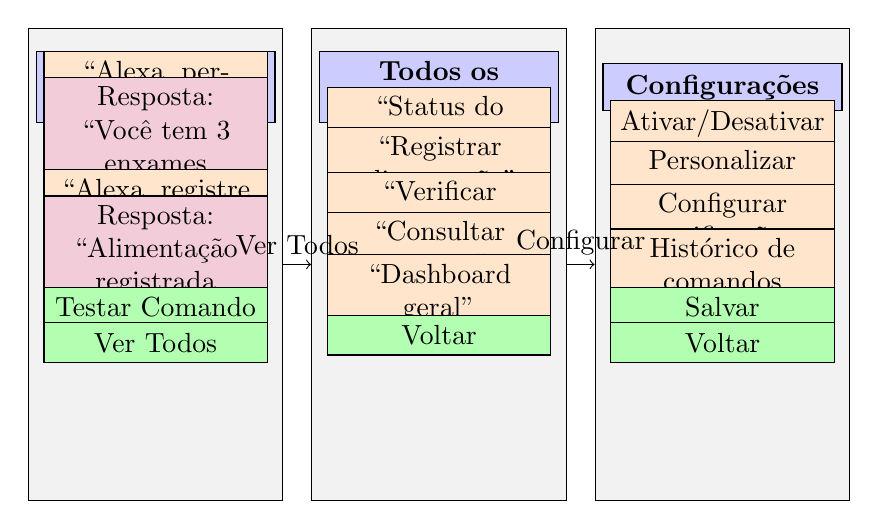
\begin{tikzpicture}[scale=0.9]
% Definição de estilos
\tikzset{
  phone/.style={rectangle, draw, fill=gray!10, text width=3cm, text centered, minimum height=6cm},
  header/.style={rectangle, draw, fill=blue!20, text width=2.8cm, text centered, minimum height=0.6cm},
  button/.style={rectangle, draw, fill=green!30, text width=2.6cm, text centered, minimum height=0.5cm},
  command/.style={rectangle, draw, fill=orange!20, text width=2.6cm, text centered, minimum height=0.4cm},
  response/.style={rectangle, draw, fill=purple!20, text width=2.6cm, text centered, minimum height=0.4cm}
}

% Tela 1: Comandos de Exemplo
\node[phone] (tela1) at (0,0) {};
\node[header] (header1) at (0,2.5) {\textbf{Comandos Alexa}};
\node[command] (cmd1) at (0,1.8) {\textquotedblleft Alexa, pergunte ao\\Pollen sobre meus\\enxames\textquotedblright};
\node[response] (resp1) at (0,1.2) {Resposta: \textquotedblleft Você tem 3\\enxames ativos. O\\enxame 1 está forte\textquotedblright};
\node[command] (cmd2) at (0,0.6) {\textquotedblleft Alexa, registre\\alimentação no\\enxame 1\textquotedblright};
\node[response] (resp2) at (0,0.0) {Resposta: \textquotedblleft Alimentação\\registrada com sucesso\textquotedblright};
\node[button] (btn1) at (0,-0.6) {Testar Comando};
\node[button] (btn2) at (0,-1.1) {Ver Todos};

% Tela 2: Lista de Comandos
\node[phone] (tela2) at (4,0) {};
\node[header] (header2) at (4,2.5) {\textbf{Todos os Comandos}};
\node[command] (cmd3) at (4,2.0) {\textquotedblleft Status do enxame\textquotedblright};
\node[command] (cmd4) at (4,1.4) {\textquotedblleft Registrar alimentação\textquotedblright};
\node[command] (cmd5) at (4,0.8) {\textquotedblleft Verificar colheita\textquotedblright};
\node[command] (cmd6) at (4,0.2) {\textquotedblleft Consultar manejo\textquotedblright};
\node[command] (cmd7) at (4,-0.4) {\textquotedblleft Dashboard geral\textquotedblright};
\node[button] (btn3) at (4,-1.0) {Voltar};

% Tela 3: Configurações
\node[phone] (tela3) at (8,0) {};
\node[header] (header3) at (8,2.5) {\textbf{Configurações}};
\node[command] (cmd8) at (8,1.8) {Ativar/Desativar\\comandos};
\node[command] (cmd9) at (8,1.2) {Personalizar\\respostas};
\node[command] (cmd10) at (8,0.6) {Configurar\\notificações};
\node[command] (cmd11) at (8,0.0) {Histórico de\\comandos};
\node[button] (btn4) at (8,-0.6) {Salvar};
\node[button] (btn5) at (8,-1.1) {Voltar};

% Setas de navegação
\draw[->] (tela1) -- node[above] {Ver Todos} (tela2);
\draw[->] (tela2) -- node[above] {Configurar} (tela3);

\end{tikzpicture}
\label{fig:wireframe-comandos-alexa}
\end{figura}

A Figura \ref{fig:wireframe-todos-comandos} exibe a tela com a listagem completa de todos os comandos de voz disponíveis na integração, permitindo que o usuário conheça todas as funcionalidades acessíveis por voz. Já a Figura \ref{fig:wireframe-desconectar-alexa} apresenta a interface para desconectar a integração com a Alexa, caso o usuário deseje revogar as permissões concedidas.

\secao{Fluxo de Processamento do Sistema}
\label{sec:fluxo-processamento}

Esta seção apresenta o processo de execução de comandos de voz na integração Alexa, detalhando o fluxo desde o comando do usuário até a resposta final.

\subsecao{Processo de Execução de Comandos de Voz}

O Quadro a seguir descreve de forma estruturada o processo completo de processamento de comandos de voz, desde a captura até a resposta ao usuário.

% BPMN - Processo de Comandos de Voz Alexa
\begin{figura}{BPMN - Processo de execução de comandos de voz na integração Alexa}{O Autor}
\centering
\begin{tikzpicture}[scale=0.8]
% Definição de estilos
\tikzset{
  start/.style={circle, draw, fill=green!20, text width=1cm, text centered, minimum height=1cm},
  end/.style={circle, draw, fill=red!20, text width=1cm, text centered, minimum height=1cm},
  process/.style={rectangle, draw, fill=blue!20, text width=2.5cm, text centered, minimum height=0.8cm},
  decision/.style={diamond, draw, fill=yellow!20, text width=2cm, text centered, minimum height=0.8cm},
  gateway/.style={diamond, draw, fill=gray!20, text width=1.5cm, text centered, minimum height=0.8cm},
  note/.style={rectangle, draw, fill=white, text width=2.5cm, text centered, minimum height=0.6cm}
}

% Eventos de início e fim
\node[start] (start) at (0,8) {Início};
\node[end] (end) at (0,0) {Fim};

% Processos principais
\node[process] (voice_input) at (0,7) {Usuário fala\\comando para Alexa};
\node[process] (alexa_process) at (0,6) {Alexa processa\\comando de voz};
\node[process] (intent_recognition) at (0,5) {Reconhecimento de\\intenção (NLP)};
\node[decision] (valid_intent) at (0,4) {Intenção\\válida?};

% Processos de validação
\node[process] (auth_check) at (-3,3) {Verificar\\autenticação};
\node[process] (permission_check) at (3,3) {Verificar\\permissões};

% Gateway de paralelização
\node[gateway] (parallel_gateway) at (0,2.5) {+};

% Processos de execução
\node[process] (api_call) at (-3,1.5) {Chamar API\\Pollen};
\node[process] (data_processing) at (3,1.5) {Processar\\dados};

% Gateway de sincronização
\node[gateway] (sync_gateway) at (0,0.8) {+};

% Processos de resposta
\node[process] (format_response) at (0,0.4) {Formatar\\resposta SSML};

% Processos de erro
\node[process] (error_handling) at (-4,2) {Tratar erro\\e informar usuário};
\node[process] (help_response) at (4,2) {Fornecer ajuda\\sobre comandos};

% Fluxos principais
\draw[->] (start) -- (voice_input);
\draw[->] (voice_input) -- (alexa_process);
\draw[->] (alexa_process) -- (intent_recognition);
\draw[->] (intent_recognition) -- (valid_intent);

% Fluxos de decisão
\draw[->] (valid_intent) -- node[above] {Sim} (parallel_gateway);
\draw[->] (valid_intent) -- node[left] {Não} (help_response);

% Fluxos paralelos
\draw[->] (parallel_gateway) -- (auth_check);
\draw[->] (parallel_gateway) -- (permission_check);

% Fluxos de sincronização
\draw[->] (auth_check) -- (sync_gateway);
\draw[->] (permission_check) -- (sync_gateway);

% Fluxos de execução
\draw[->] (sync_gateway) -- (api_call);
\draw[->] (sync_gateway) -- (data_processing);

% Fluxo final
\draw[->] (api_call) -- (format_response);
\draw[->] (data_processing) -- (format_response);
\draw[->] (format_response) -- (end);

% Fluxos de erro
\draw[->] (help_response) -- (end);
\draw[->] (error_handling) -- (end);

% Anotações
\node[note] (note1) at (-5,6) {Comando: \textquotedblleft Alexa, pergunte\\ao Pollen sobre\\meus enxames\textquotedblright};
\node[note] (note2) at (5,4) {Exemplo de intenções:\\• ConsultarStatus\\• RegistrarAlimentacao\\• VerificarColheita};
\node[note] (note3) at (-5,1) {API REST:\\GET /enxame/user/\{id\}\\POST /alimentacao};
\node[note] (note4) at (5,1) {Processamento:\\• Validação de dados\\• Formatação de resposta\\• Geração de SSML};

\end{tikzpicture}
\label{fig:bpmn-comandos-voz}
\end{figura}

O Quadro \ref{quad:fluxo-comandos-voz} apresenta as sete etapas do processo de execução de comandos de voz na integração Alexa+Pollen. O processo inicia com a captura do comando de voz pelo dispositivo Alexa, passa pelo reconhecimento de linguagem natural (NLP), validação do comando e autenticação do usuário. Após a autenticação bem-sucedida, o sistema realiza a chamada à API do Pollen para buscar os dados solicitados, processa esses dados formatando-os em SSML (Speech Synthesis Markup Language) e, finalmente, a Alexa retorna a resposta em voz ao usuário. Este fluxo garante que apenas usuários autenticados possam acessar informações sensíveis e que comandos inválidos sejam tratados adequadamente com mensagens de ajuda.

\secao{Considerações Finais do Capítulo}

A solução planejada representa uma integração inovadora entre assistentes virtuais e aplicações de gestão apícola, oferecendo aos apicultores uma forma eficiente e hands-free de acessar informações sobre suas colmeias durante o trabalho no apiário.

Os artefatos de planejamento apresentados neste capítulo demonstram a viabilidade técnica da integração proposta. O Diagrama de Caso de Uso ilustra as funcionalidades principais e as interações entre os atores do sistema. Os Quadros de estrutura de dados definem as entidades e relacionamentos que serão utilizados pela integração. Os Wireframes apresentam as interfaces de configuração que serão disponibilizadas aos usuários no aplicativo Pollen. Por fim, o Quadro de Processo de Comandos de Voz detalha as sete etapas de execução desde o comando até a resposta.

O planejamento apresentado atende aos requisitos funcionais e não funcionais definidos na Seção \ref{sec:requisitos-sistema}, proporcionando uma base sólida para a futura implementação da solução no TCC 02. A integração planejada contribuirá significativamente para a eficiência da gestão apícola, permitindo acesso à informação através de comandos de voz naturais em português brasileiro.